\documentclass[12pt,a4paper,t,xcolor=dvipsnames,slidestop,compress,mathserif]{beamer}
\usepackage{amsmath,amssymb,graphicx,color,multicol,amsfonts,algorithmic,url,stmaryrd,epsf}
\usepackage{graphicx, algorithm2e}

%% ----------------------------------------------------------------------
%% Definitions, Macros, Etc.
%% ----------------------------------------------------------------------

%% Hyper-linked References
\newcommand{\Sec}[1]{\hyperref[sec:#1]{\S\ref*{sec:#1}}} %section
\newcommand{\Eqn}[1]{\hyperref[eq:#1]{(\ref*{eq:#1})}} %equation
\newcommand{\Fig}[1]{\hyperref[fig:#1]{Figure~\ref*{fig:#1}}} %figure
\newcommand{\Tab}[1]{\hyperref[tab:#1]{Table~\ref*{tab:#1}}} %table
\newcommand{\Thm}[1]{\hyperref[thm:#1]{Theorem~\ref*{thm:#1}}} %theorem
\newcommand{\Lem}[1]{\hyperref[lem:#1]{Lemma~\ref*{lem:#1}}} %lemma
\newcommand{\Prop}[1]{\hyperref[prop:#1]{Property~\ref*{prop:#1}}} %property
\newcommand{\Cor}[1]{\hyperref[cor:#1]{Corollary~\ref*{cor:#1}}} %corollary
\newcommand{\Def}[1]{\hyperref[def:#1]{Definition~\ref*{def:#1}}} %definition
\newcommand{\Alg}[1]{\hyperref[alg:#1]{Algorithm~\ref*{alg:#1}}} %algorithm
\newcommand{\Ex}[1]{\hyperref[ex:#1]{Example~\ref*{ex:#1}}} %example

% Theorem-like constructs
%\newtheorem{example}[theorem]{Example}

% Blackboard fonts 
\newcommand{\Real}{\mathbb{R}}
\newcommand{\Cplx}{\mathbb{C}}
%% Transposes
\newcommand{\Tra}{^{\rm T}} % Transpose
\newcommand{\Cct}{^\dagger} % Complex conjugate transpose

%% Permutation index
\newcommand{\bfpp}{{\bf p}_n}

%% Matrix & Tensor Operations
\newcommand{\Circ}[1]{{\rm circ}\left( #1 \right)}
\newcommand{\Fold}[1]{{\rm fold}\left( #1 \right)}
\newcommand{\Unfold}[1]{{\rm unfold}\left( #1 \right)}
\newcommand{\Twist}[1]{{\rm twist}(\M{#1})}
\newcommand{\Squeeze}[1]{{\rm squeeze}(#1)}
\newcommand{\squeeze}{{\rm squeeze}}
\newcommand{\Mout}{\diamondsuit}
\newcommand{\circu}{ {\rm circ}}
\newcommand{\bcirc}{ {\rm circ}}
\newcommand{\vvec}{ {\rm vec}}

\newcommand{\mc}[1]{\mathcal{#1}}
\newcommand{\mb}[1]{\mathbb{#1}}
\newcommand{\mcr}[1]{\mathrsfs{#1}}

%% Element of complicated object that is surrounded by parens
\newcommand{\PE}[2]{\left( #1 \right)_{#2}}

%% Vector notation
\newcommand{\V}[1]{{\bm{\mathbf{\MakeLowercase{#1}}}}} % vector
\newcommand{\VE}[2]{\MakeLowercase{#1}_{#2}} % vector element

%% Matrix notation
\newcommand{\M}[1]{{\bm{\mathbf{\MakeUppercase{#1}}}}} % matrix
\newcommand{\Mhat}[1]{{\bm{\hat \mathbf{\MakeUppercase{#1}}}}} % matrix
\newcommand{\Mbar}[1]{{\bm{\bar \mathbf{\MakeUppercase{#1}}}}} % matrix
\newcommand{\ME}[2]{\MakeLowercase{#1}_{#2}} % matrix element
\newcommand{\MC}[2]{\V{#1}_{#2}}

%% Tensor notation
\newcommand{\T}[1]{\boldsymbol{\mathscr{\MakeUppercase{#1}}}} %tensor
\newcommand{\TLS}[2]{\M{#1}_{[#2]}} % lateral slice
\newcommand{\TFS}[2]{\M{#1}_{#2}} % frontal slice
\newcommand{\TT}[2]{\V{#1}_{#2}} % tube
\newcommand{\TE}[2]{\MakeLowercase{#1}_{#2}} % tensor element


%% Shortcuts
\newcommand{\TA}{\T{A}}
\newcommand{\TB}{\T{B}}
\newcommand{\TS}{\T{S}}
\newcommand{\TC}{\T{C}}
\newcommand{\TU}{\T{U}}
\newcommand{\TV}{\T{V}}
\newcommand{\TG}{\T{G}}

\newcommand{\Vu}{\V{u}}
\newcommand{\Vv}{\V{v}}
\newcommand{\Vq}{\V{q}}
\newcommand{\Vr}{\V{r}}
\newcommand{\Vp}{\V{p}}
\newcommand{\Vd}{\V{d}}
\newcommand{\Vz}{\V{z}}
\newcommand{\Vb}{\V{b}}
\newcommand{\Vg}{\V{g}}
\newcommand{\Vh}{\V{h}}
\newcommand{\MH}{\M{H}}
\newcommand{\MG}{\M{G}}
\newcommand{\MA}{\M{A}}
\newcommand{\MX}{\M{X}}
\newcommand{\MZ}{\M{Z}}
\newcommand{\MW}{\M{W}}
%\newcommand{\TD}{\T{D}}

\newcommand{\SaS}{{\mathcal S}}

\newcommand{\MGC}{\tilde{\MG}}

\newcommand{\Matlab}{{\sc Matlab}\xspace}
\newcommand{\matlab}{{\sc Matlab}\xspace}
\newcommand{\qtext}[1]{\quad\text{#1}\quad}

\newcommand{\matvec}{{\tt Vec}}
\newcommand{\fld}{{\tt Fold}}

\def \bK{\mathbf{K}}
\def \bF{\mathbf{F}}
\def \bD{\mathbf{D}}
\def \bB{\mathbf{B}}
\def \bA{\mathbf{A}}
\newcommand{\bDelta}{\boldsymbol{\Delta}}

%\newcommand{\bea}{\left[ \begin{array}}
%\newcommand{\eea}{ \end{array} \right]} 

\newcommand{\bftheta}{ {\boldsymbol \theta}}
\newcommand{\bfrho}{ {\boldsymbol \rho}}
\newcommand{\bfeta}{ {\boldsymbol \eta}}
\newcommand{\fft}{ \mbox{\tt fft} }
\newcommand{\ifft}{ \mbox{\tt ifft} }
\newcommand{\blkd}{\mbox{\tt blkdiag}}
\newcommand{\rshpT}{\mbox{\tt reshapeT}}
\newcommand{\F}[1]{\mathcal{F}\{#1\}}
\newcommand{\Fi}[1]{\mathcal{F}^{-1}\{#1\}}
\newcommand{\indep}{\perp\!\!\!\perp}

\usepackage{mathtools}
\DeclarePairedDelimiter{\ceil}{\lceil}{\rceil}
\DeclarePairedDelimiter{\floor}{\lfloor}{\rfloor}
\newcommand{\Var}{\text{Var}}
\newcommand{\E}{\text{E}}
\newcommand{\Cov}{\text{Cov}}



%\usepackage{beamerthemesplit}

\setlength{\columnsep}{1pt}


\newcommand{\A}{A}%{\mathbb{A}}
\newcommand{\Mff}{M_{ff}}
\newcommand{\Mffinv}{M_{ff}^{-1}}
\newcommand{\Aff}{A_{ff}}
\newcommand{\Affinv}{A_{ff}^{-1}}
\newcommand{\Aschur}{\hat{A}_{cc}}
\newcommand{\Aschurinv}{\hat{A}_{cc}^{-1}}
\newcommand{\Afc}{A_{fc}}
\newcommand{\Acf}{A_{cf}}
\newcommand{\Acc}{A_{cc}}
\newcommand{\half}{\frac{1}{2}}
\DeclareMathOperator*{\argmin}{argmin}
\renewcommand{\H}[1]{{#1}^\star}

% Beamer Commands
\setbeamertemplate{navigation symbols}{}
%\setbeamertemplate{footline}
%{%
%\hspace*{0.55\linewidth}\insertshorttitle - p.\insertframenumber
%}
%\setbeamertemplate{footnote}

%{%\insertfootnotetext}
\setbeamercolor{footnote mark}{fg=white}
\setbeamertemplate{frametitle}[default][center]
\setbeamertemplate{itemize item}[circle]
\setbeamertemplate{itemize subitem}[triangle]
\setbeamercolor{itemize subitem}{fg=Plum}
\setbeamerfont{itemize subitem}{size=\normalsize}
\setbeamercolor{alerted text}{fg=Magenta}
\setbeamerfont{institute}{size=\normalsize}
\setbeamerfont{list label}{series=\bfseries}
\usefonttheme[onlylarge]{structurebold} 

%%%%%%%%%%%%%%%%%%%%%%%%%%%%%%%%%%%%%%%%%%%%%%%%% include packages

\usetheme{Madrid}
%% For \mathscr
\usepackage[mathscr]{eucal}

\usepackage{amssymb}

%% For \boldsymbol
\usepackage{amsbsy}

%% For \bm (bold math)
\usepackage{bm}

%% For special lists like inparaenum, compactenum, compactitem
\usepackage{paralist}

%% For xspace (intelligent spacing at the end of a macro)
\usepackage{xspace}

\usepackage{centernot}
\usepackage{pdfpages}

%%%%%%%%%%%%%%
%colors
%%%%%%%%%%%%
\newcommand{\red}[1]{{\color{red}#1}}
\newcommand{\green}[1]{{\color{green}#1}}
\newcommand{\yellow}[1]{{\color{yellow}#1}}
\newcommand{\blue}[1]{{\color{blue}#1}}


% Title Page Stuff
% Title Page Stuff
\title[Likelihood-free MCMC]{Parameter inference for small biochemical systems using likelihood-free MCMC}
\author[Eric Kernfeld]{ {Eric Kernfeld}\inst{1}}
\institute[University of Washington]
{ \inst{1}%
University of Washington Department of Statistics}
\date{}


\begin{document}

% Title Page
% - Begin Slide -----
\maketitle

%\begin{frame}
%\frame{\tableofcontents}
% Collaborators/support
% - Begin Slide -----
%\section[Notation]{Background and Notations}

%%%%%%%%%%%%%%%%%%%%%%%%%%%%%%%%%%%%%%%%
%\begin{frame}{Outline}
%\tableofcontents
%\end{frame}

%%%%%%%%%%%%%%%%%%%%%%%%%%%%%%%%%%%%%%%%%
\begin{frame}{Paper}
Darren Wilkinson's ``Parameter inference for stochastic kinetic models of bacterial gene regulation,'' a chapter of the proceedings in \cite{Bernardo2012}.

\end{frame}
%%%%%%%%%%%%%%%%%%%%%%%%%%%%%%%%%%%%%%%%%
%\begin{frame}{Problem}
%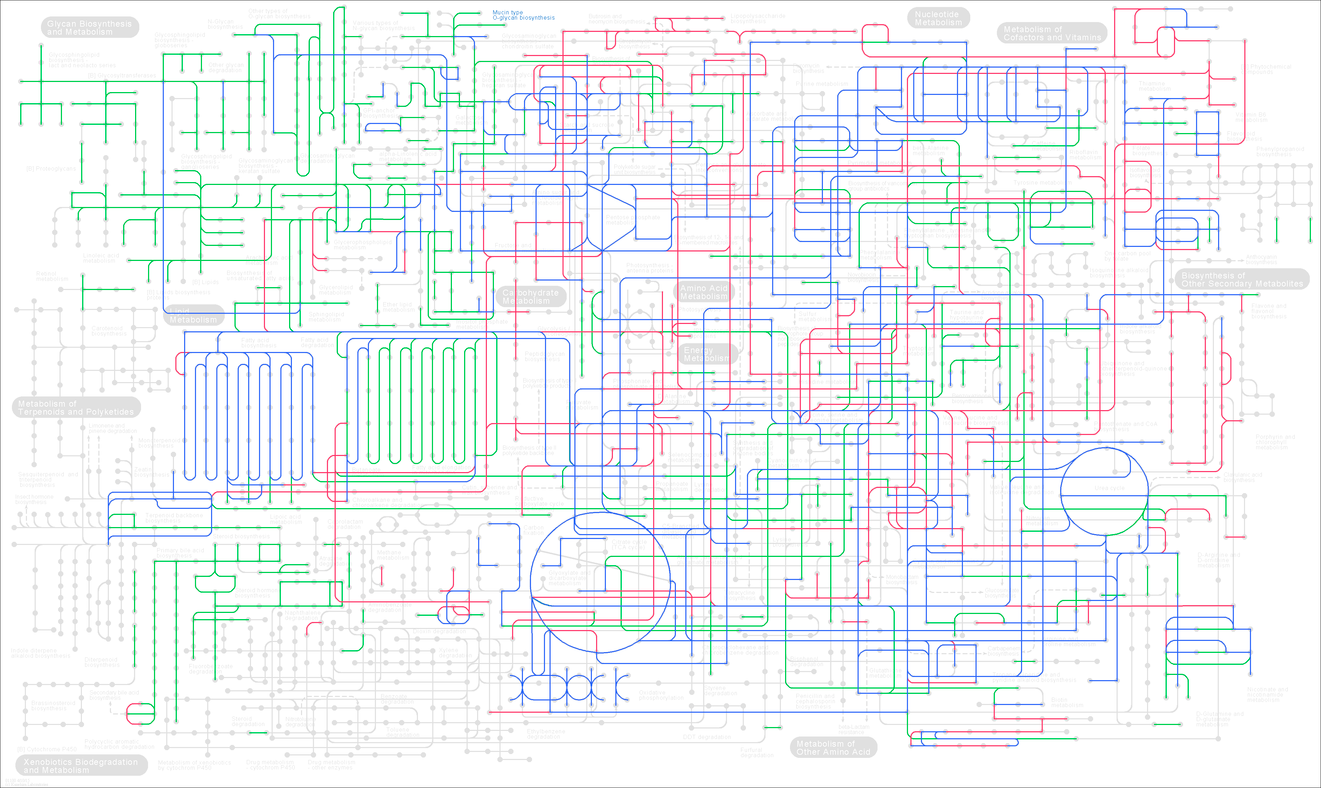
\includegraphics[scale=0.25]{human_metabolism_kegg.png}
%\end{frame}

%%%%%%%%%%%%%%%%%%%%%%%%%%%%%%%%%%%%%%%%%
\begin{frame}{Problem}

Cast of Characters 
\begin{itemize}
\item Simulation begins at time $0$ and proceeds in continuous time.
\item $\mathcal{R}_j$ is a chemical reaction.
\item $R_j(t) \in \mathbb{Z}_{\geq 0}$ counts occurrences of $\mathcal{R}_j$ up to time $t$.
\item $\theta_j\in \mathbb{R}_{\geq 0}$ is the rate at which $\mathcal{R}_j$ happens. More on this in future slides.
\item $X_i(t)  \in \mathbb{Z}_{\geq 0}$ is the number of molecules of type $i$
\item $\mathcal{D}_t \in \mathbb{R}$ is an incomplete observation of $X(t)$ with error.
\end{itemize}

\end{frame}
%%%%%%%%%%%%%%%%%%%%%%%%%%%%%%%%%%%%%%%%%
\begin{frame}{Problem}
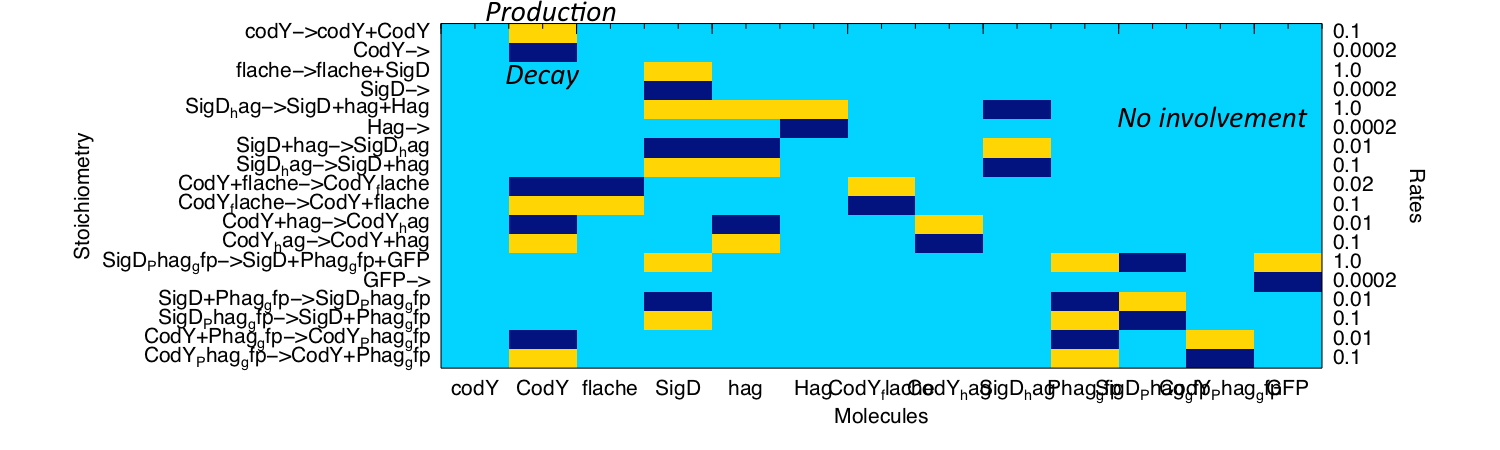
\includegraphics[scale=0.35]{stoich_fig.png}
$$R_3(t)\sim PP(\theta_3{X_1(t)\choose1}{X_2(t)\choose1}{X_3(t)\choose1})$$
Assume reaction $\mathcal{R}_j$ occurs independently of other patterns except when the contents of the system changes.
\end{frame}
%%%%%%%%%%%%%%%%%%%%%%%%%%%%%%%%%%%%%%%%%
\begin{frame}{Problem}
Given $\mathcal{D}_t$, find $c$. 
\pause
Also, switching to ODE's is not allowed: stochastic models are biologically necessary (\cite{reinker2006parameter} and references therein).
\end{frame}

%%%%%%%%%%%%%%%%%%%%%%%%%%%%%%%%%%%%%%%%%
\begin{frame}{Problem}
Likelihood: $$P(X(\vec{t}), \vec{t}|c) = \prod_{i=1}^n c_{\nu_{i}} \prod_{j=1}^u {{X_{j}(t_{i-1})}\choose{p_{{\nu_{i}}j}}}\exp\left(-c_{\nu_{i}}\int_0^T {{X_j(t)}\choose{p_{{\nu_{i}}j}}} dt\right)$$
\end{frame}

%%%%%%%%%%%%%%%%%%%%%%%%%%%%%%%%%%%%%%%%%
\begin{frame}{Other work}
\begin{itemize} 
\item Approximate MJP with SDE \cite{golightly2005bayesian,bayes_stoch_mod,fearnhead2014inference}

\item Method of moments \cite{milner2013moment,zechner2012moment}

\item Variational inference with mean-field approximation  \cite{opper2008variational} 

\item Approximate Bayesian Computation (ABC) and MCMC
\cite{owen2014ABC_LF-MCMCcomparison,owen2014scalable,hobolth2009simulation,zechner2014scalable}


\item EM with a sample average replacing the E-step expectation or similar \cite{gupta2014comparison,srivastava_rawlings2014stoch_opt,bayer2015stoch_em,horvath2008parameter,daigle2012accelerated}
\end{itemize}


\end{frame}
%%%%%%%%%%%%%%%%%%%%%%%%%%%%%%%%%%%%%%%%%
\begin{frame}{Likelihood Free MCMC}

To produce a chain of samples from $P(\theta|D)$, using a proposal $q(\theta^*|\theta)$, accept with probability $p_{rej}(\theta^*|\theta)\equiv\min \{1, A\}$ if $$A=\frac{q(\theta,x|\theta^*,x^*)}{q(\theta^*,x^*|\theta,x)} \times \frac{P(\theta^*,x^*|\mathcal{D})}{P(\theta,x|\mathcal{D})}
$$
%.$$ or equivalently$$A{q(\theta^*|\theta)}{P(\theta|D)}={q(\theta|\theta^*)}  {P(\theta^*|D)}.$$ 

\end{frame}
%%%%%%%%%%%%%%%%%%%%%%%%%%%%%%%%%%%%%%%%%%
%\begin{frame}{Likelihood Free MCMC}
%
%Cast of Characters (\red{things DW can't evaluate are in red})
%\begin{itemize}
%\item ${P(\theta)}$
%\item \red{${P(x|\theta)}$}
%\item ${P(\mathcal{D}|x, \theta)}$
%\item \red{${P(x, \theta|\mathcal{D})}$} 
%\end{itemize}
%
%$$A=\frac{q(\theta,x|\theta^*,x^*)}{q(\theta^*,x^*|\theta,x)} \times \frac{P(\theta^*,x^*|\mathcal{D})}{P(\theta,x|\mathcal{D})}.$$ 
%
%
%\end{frame}

%%%%%%%%%%%%%%%%%%%%%%%%%%%%%%%%%%%%%%%%%
\begin{frame}{Likelihood Free MCMC}

\begin{align*}
&\frac{q(\theta^*, x^*|\theta, x)}{q(\theta, x|\theta^*, x^*)}
\times 
\red{\frac{P(x| \theta)}{P(x^*| \theta^*)}} 
\frac{ P( \theta)}{ P( \theta^*)} 
\frac{P(\mathcal{D}|x, \theta)}{P(\mathcal{D}|x^*, \theta^*)}\\
&=\frac{f(\theta^*|\theta)}{f(\theta|\theta^*)}
\red{\frac{P(x^*| \theta^*)}{P(x| \theta)} }
\times 
\red{\frac{P(x| \theta)}{P(x^*| \theta^*)} } 
\frac{ P( \theta)}{ P( \theta^*)}
\frac{P(\mathcal{D}|x, \theta)}{P(\mathcal{D}|x^*, \theta^*)}\\
&=\frac{f(\theta^*|\theta)}{f(\theta|\theta^*)}
\times 
\frac{ P( \theta)}{ P( \theta^*)} 
\frac{P(\mathcal{D}|x, \theta)}{P(\mathcal{D}|x^*, \theta^*)}.
\end{align*}
This approach due to Marjoram et al. (paper title: ``MCMC Without Likelihoods'') \cite{Marjoram23122003}. 
\end{frame}

%%%%%%%%%%%%%%%%%%%%%%%%%%%%%%%%%%%%%%%%%
\begin{frame}{Likelihood Free Particle MCMC}
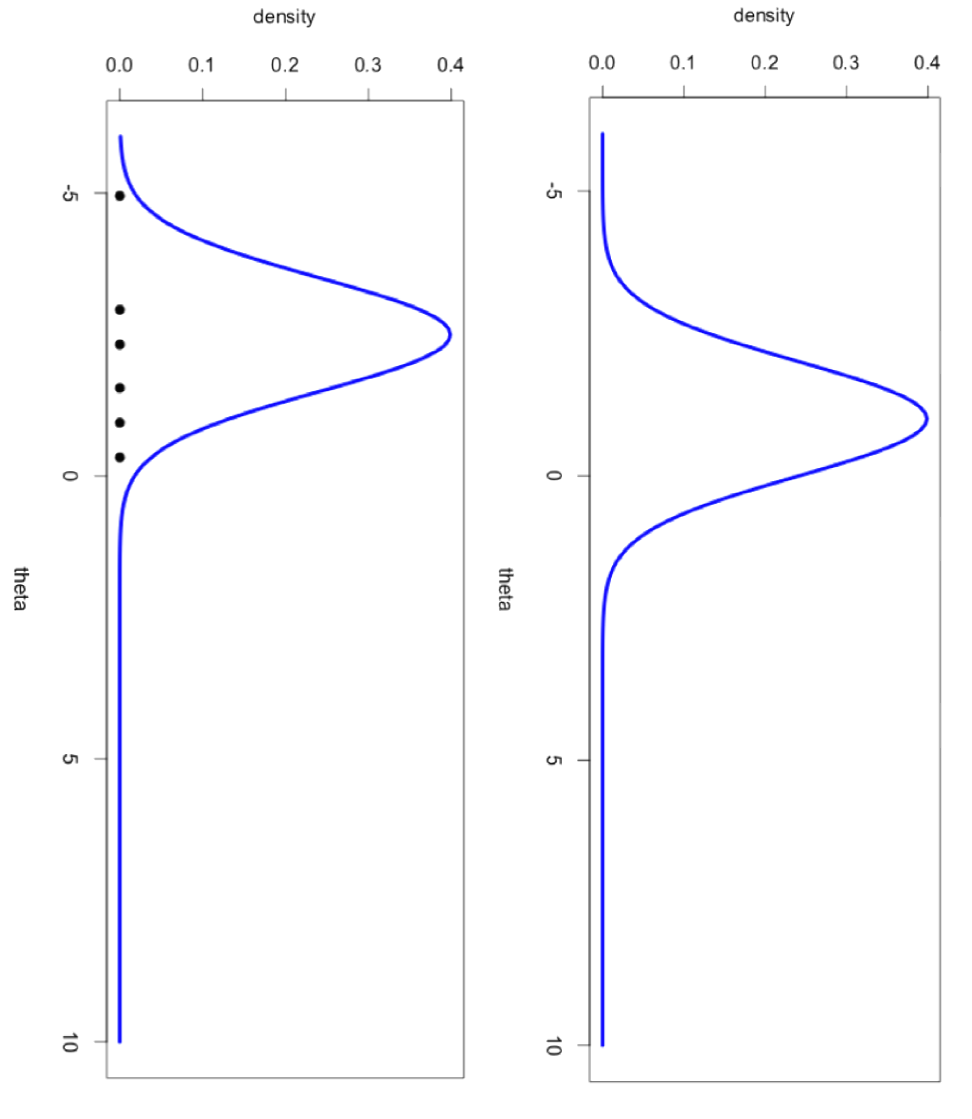
\includegraphics[scale=0.35]{prior_sample_graphic.png}
\end{frame}
\begin{frame}{Likelihood Free Particle MCMC}
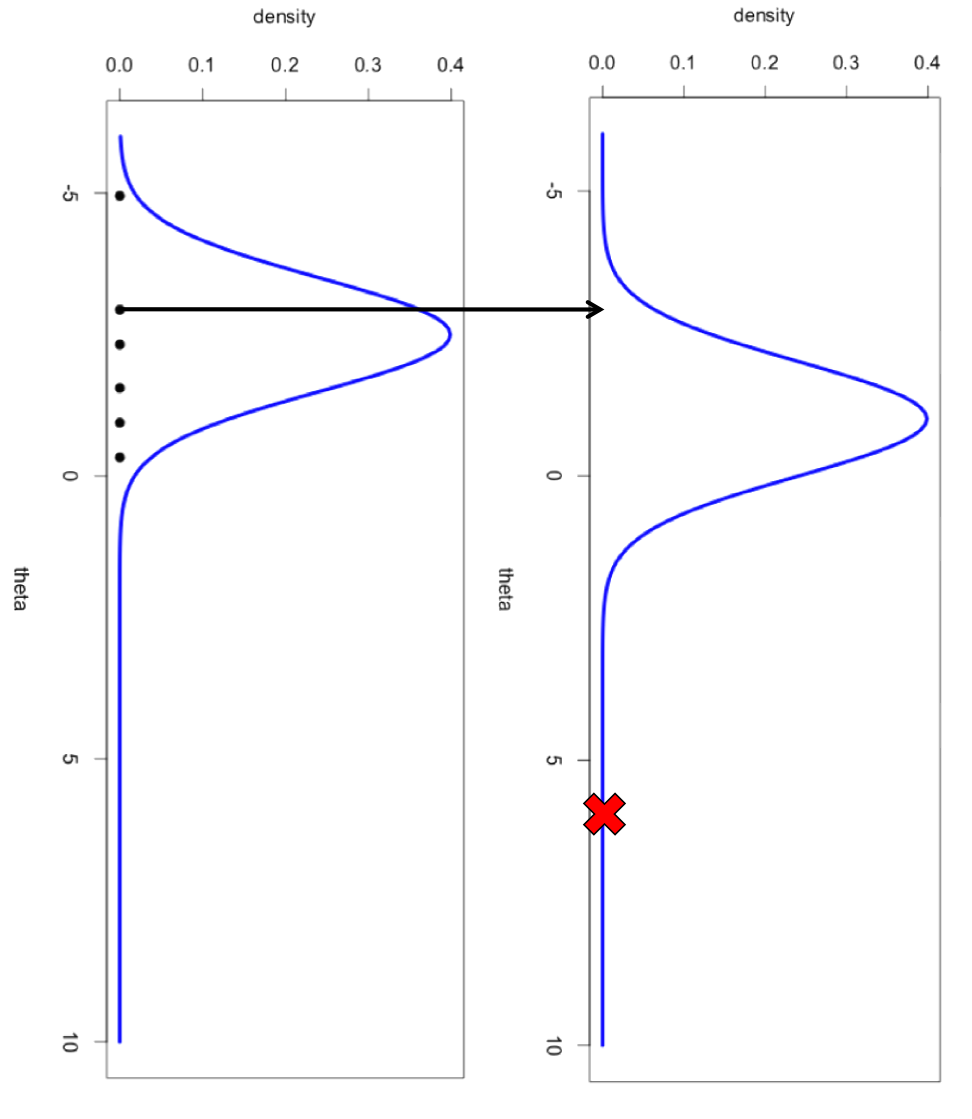
\includegraphics[scale=0.35]{post_sample1_graphic.png}
\end{frame}
\begin{frame}{Likelihood Free Particle MCMC}
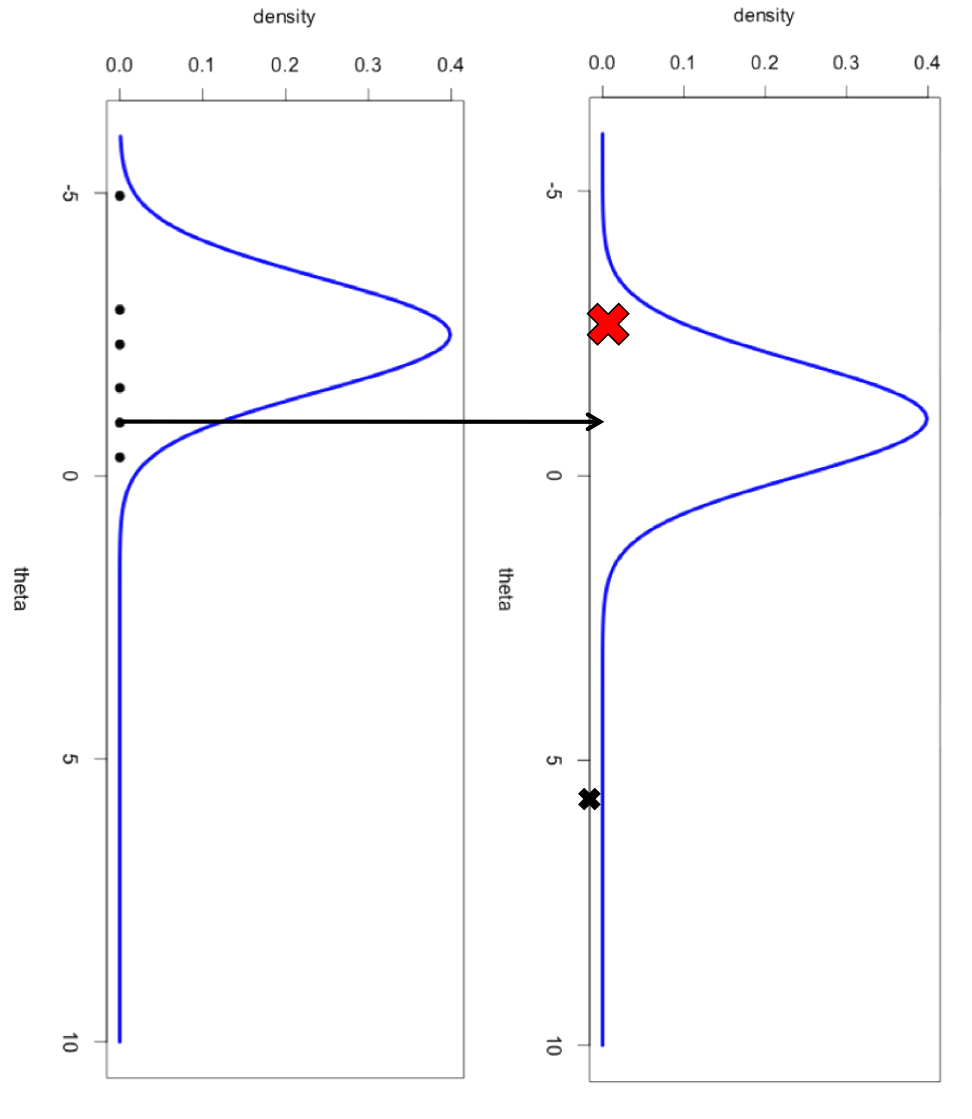
\includegraphics[scale=0.35]{post_sample2_graphic.png}
\end{frame}
\begin{frame}{Likelihood Free Particle MCMC}
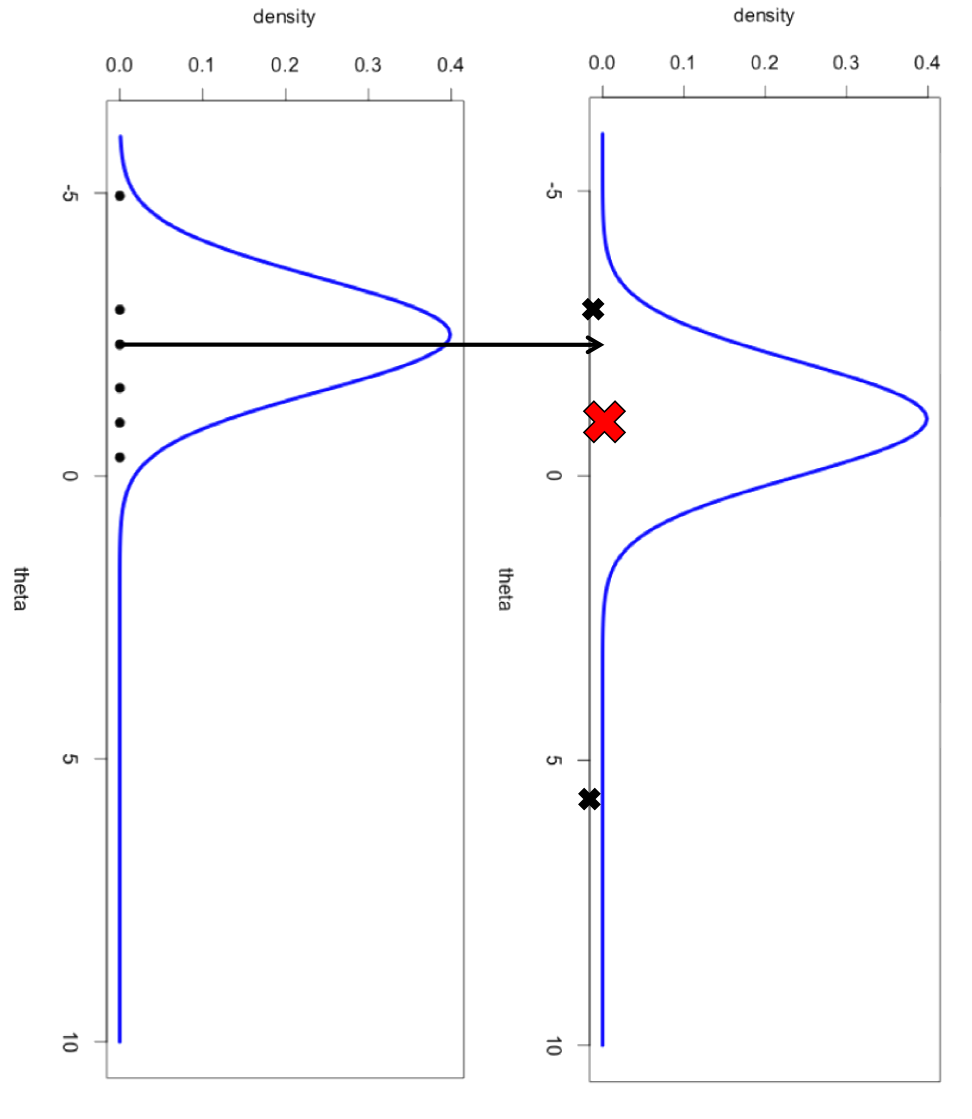
\includegraphics[scale=0.35]{post_sample3_graphic.png}
\end{frame}
\begin{frame}{Likelihood Free Particle MCMC}
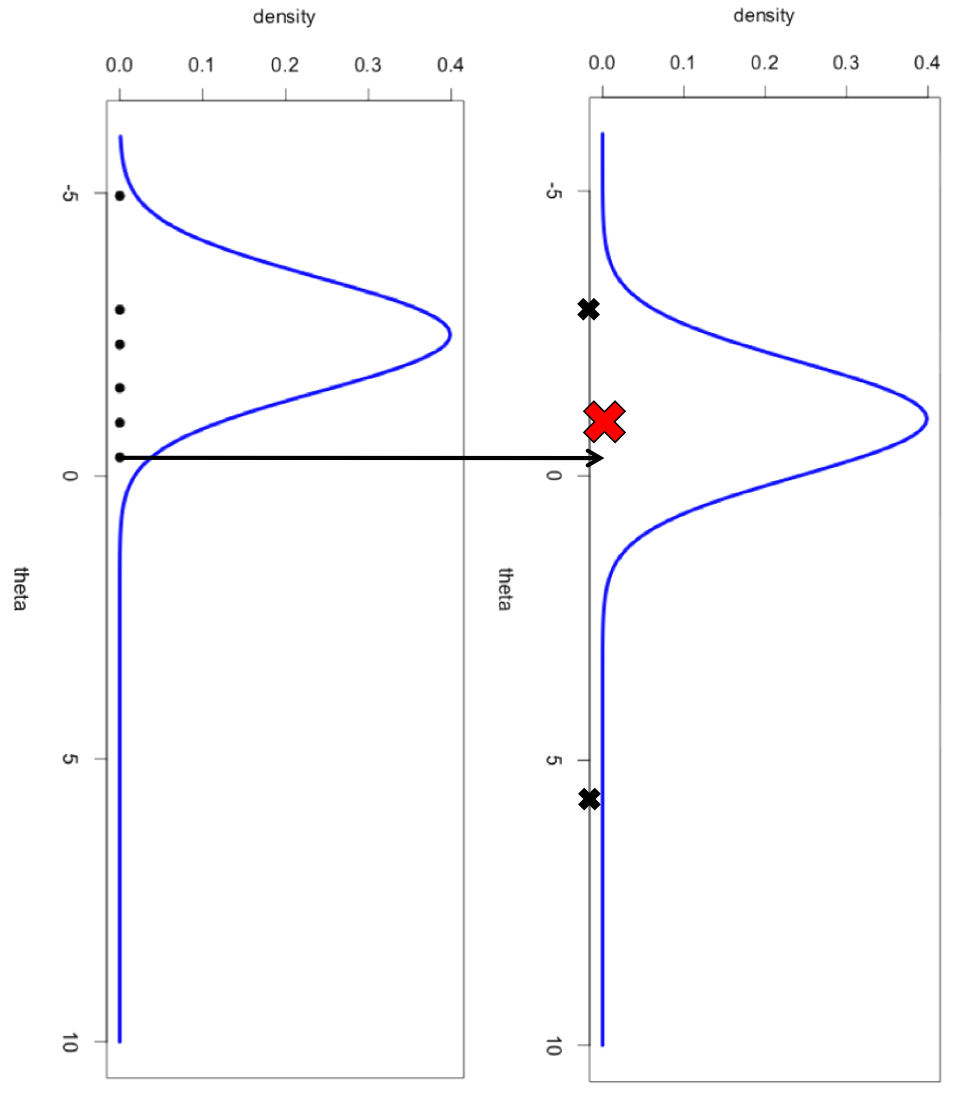
\includegraphics[scale=0.35]{post_sample4_graphic.png}
\end{frame}
\begin{frame}{Likelihood Free Particle MCMC}
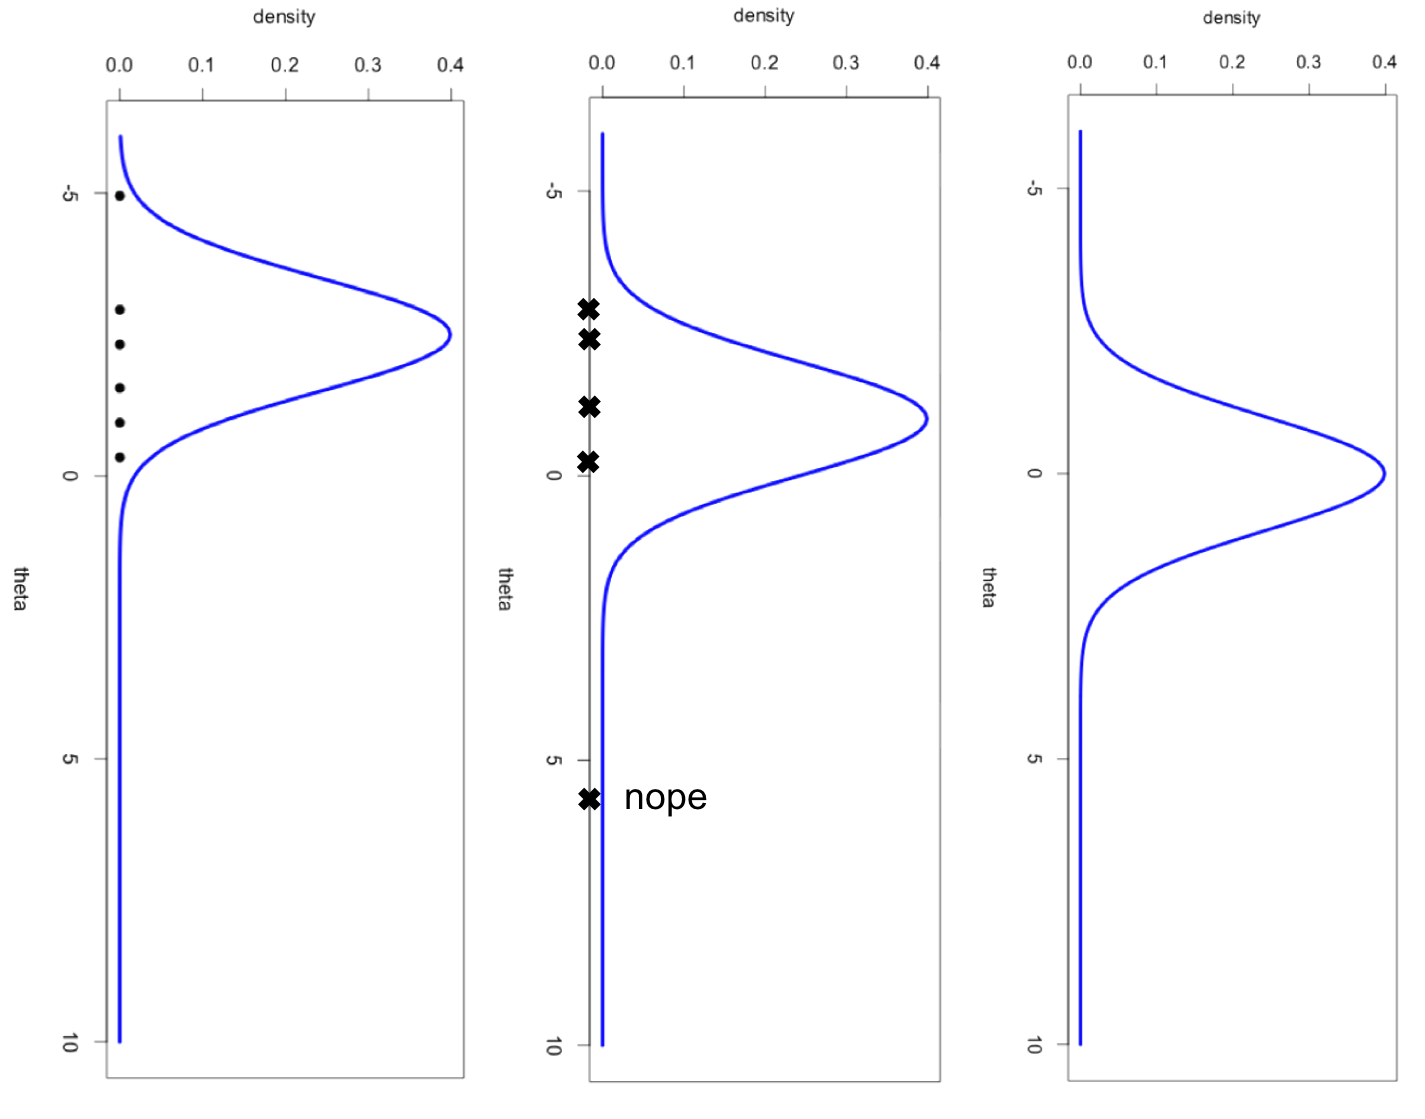
\includegraphics[scale=0.35]{post_sample5_graphic.png}
\end{frame}
\begin{frame}{Likelihood Free Particle MCMC}
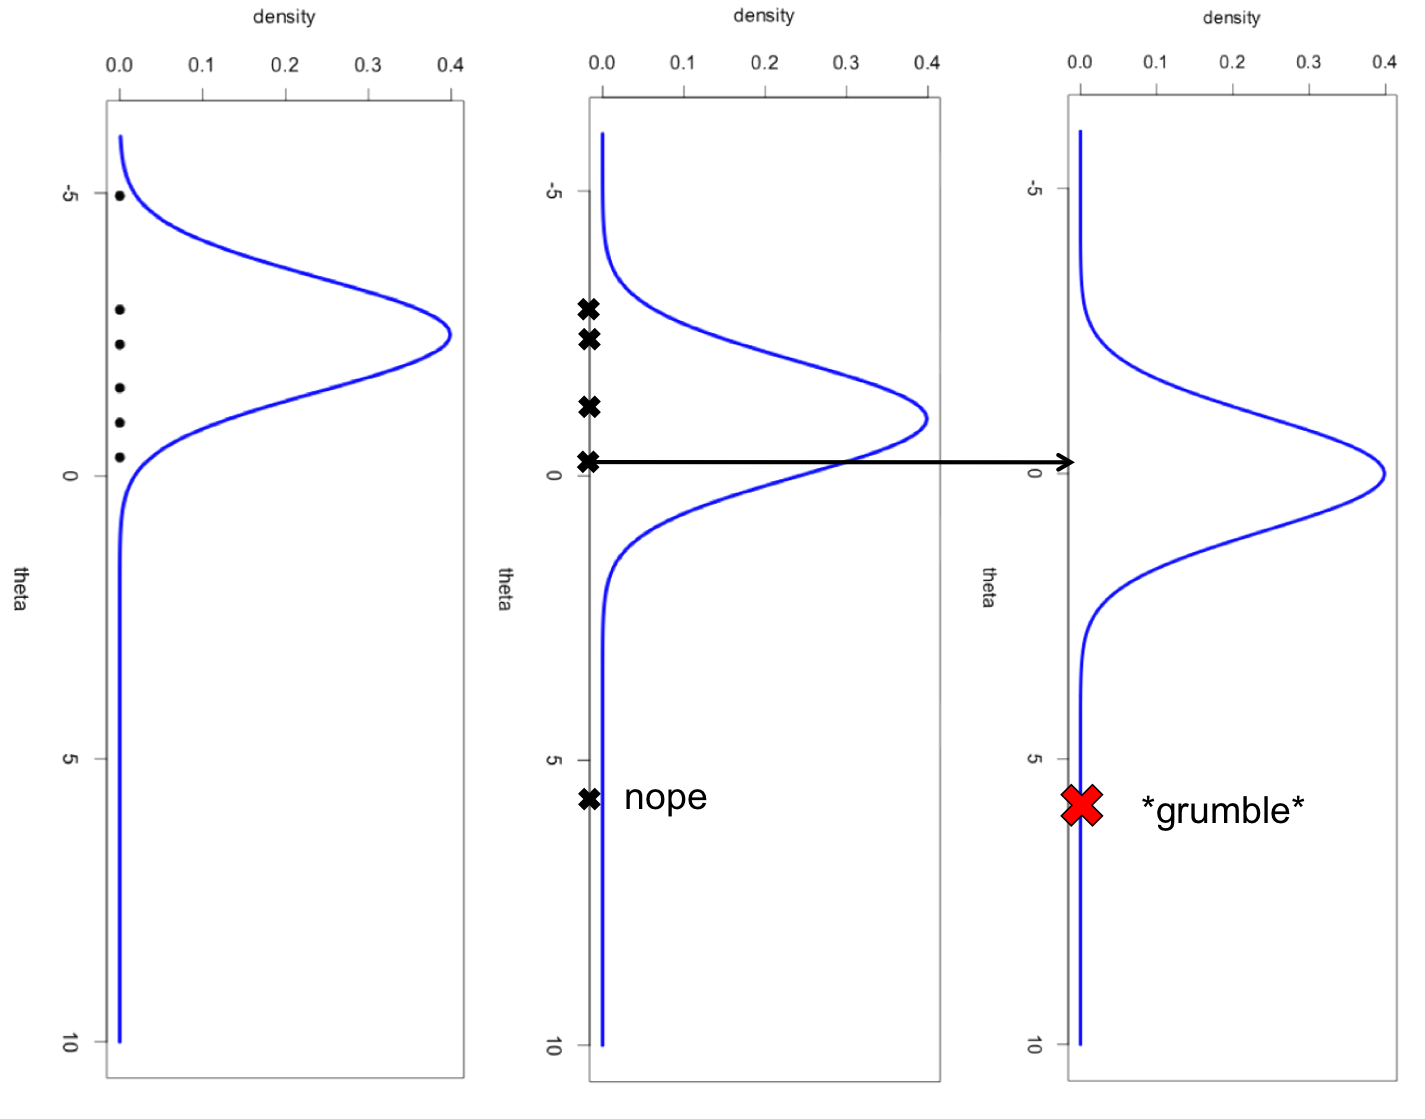
\includegraphics[scale=0.35]{post_sample6_graphic.png}
\end{frame}
%%%%%%%%%%%%%%%%%%%%%%%%%%%%%%%%%%%%%%%%%%
\begin{frame}{Likelihood Free Particle MCMC}
\begin{center}

\includegraphics[scale=0.55]{insanity_wolf.jpg}
\end{center}
\end{frame}
%%%%%%%%%%%%%%%%%%%%%%%%%%%%%%%%%%%%%%%%%%
\begin{frame}{Likelihood Free Particle MCMC}

\begin{algorithm}[H]
Given a hidden continuous-time Markov process $\{x_t\}_{t=0}^T$ with: \\
\Indp \Indp
Unknown parameters $\theta$ and known initial state $x_0$\\
Data points $\mathcal{D}_{t_{i}}$ at times $t_{i}$, $i \in \{1, ... I\}$ \\
A simple, tractable error model $P(\mathcal{D}_{t_{i}}|x_{t_{i}}, \theta)$\\
A simulator for paths of $x$ given $\theta$\\
An array $B_0$ of 1,000,000 samples from a prior on $\theta, x_0$\\
Empty arrays $B_{i}$ of the same length\\

\Indm \Indm
For each time point (for $i \in \{1, ... I\}$):\\
\Indp\Indp
Until $B_{i}$ is full: \\
\Indp\Indp
Draw $(\theta^*, x_{t_{i-1}}^*)$ from $B_{i-1}$ or a KDE of its contents\\
Using $(\theta^*, x_{t_{i-1}}^*)$, simulate up to $x_{t_{i}}^*$, the state at time $t_{i}$ \\
Set $A=\min(1, \frac{P(\mathcal{D}_{t_{i}}|x_{t_{i}}^*, \theta^*)}{P(\mathcal{D}_{t_{i}}|x_{t_{i}}, \theta)})$\\
With probability $A$, overwrite $(\theta, x_{t_{i}})$ with $(\theta^*, x_{t_{i}}^*)$\\
After burn-in and thinning, add $(\theta, x_{t_{i}})$ to $B_{i}$\\

\end{algorithm}
\end{frame}
%%%%%%%%%%%%%%%%%%%%%%%%%%%%%%%%%%%%%%%%%%
\begin{frame}{Likelihood Free Particle MCMC}
$$ \frac{P(x_{t_{i}}^*| x_{t_{i-1}}^*,\theta^*\red{, \mathcal{D}_{t_{i-1}}})}{P(x_{t_{i}}| x_{t_{i-1}}, \theta \red{, \mathcal{D}_{t_{i-1}}})} 
\frac{P(x_{t_{i-1}}^*,\theta^*| \mathcal{D}_{t_{i-1}})}{P(x_{t_{i-1}}, \theta| \mathcal{D}_{t_{i-1}})}
\times $$
$$\frac{P(x_{t_{i}}| x_{t_{i-1}}, \theta \red{, \mathcal{D}_{t_{i-1}}})}{P(x_{t_{i}}^*| x_{t_{i-1}}^*,\theta^*\red{, \mathcal{D}_{t_{i-1}}})}
\frac{ P(x_{t_{i-1}}, \theta| \mathcal{D}_{t_{i-1}})}{ P( x_{t_{i-1}}^*,\theta^*| \mathcal{D}_{t_{i-1}})}   
\frac{P(\mathcal{D}_{t_{i}}|x_{t_{i}}, \theta)}{P(\mathcal{D}_{t_{i}}|x_{t_{i}}^*, \theta^*)}$$  
\pause

$${P(x_{t_{i}}| x_{t_{i-1}}, \theta \red{, \mathcal{D}_{t_{i-1}}})}
{ P(x_{t_{i-1}}, \theta| \mathcal{D}_{t_{i-1}})}
{P(\mathcal{D}_{t_{i}}|x_{t_{i}}, \theta)}$$ \\
\pause
$$={P(x_{t_{i}}, x_{t_{i-1}}, \theta |\red{ \mathcal{D}_{t_{i-1}}})}
{P(\mathcal{D}_{t_{i}}|x_{t_{i}}, \theta, \red{ x_{t_{i-1}},\mathcal{D}_{t_{i-1}}})}$$ \\

$$={P(x_{t_{i}}, x_{t_{i-1}}, \theta |\red{ \mathcal{D}_{t_{i}}})P( \mathcal{D}_{t_{i}}| \mathcal{D}_{t_{i-1}})}$$ \\
\end{frame}
%%%%%%%%%%%%%%%%%%%%%%%%%%%%%%%%%%%%%%%%%%
%\begin{frame}{Sequential Importance Sampling}
%I learned about SIS here \cite{SMC_Doucet_Freitas_Gordon}.
%
%For (non-sequential) importance sampling, get $\int g(x, \theta)P(x, \theta|\mathcal{D})dx$ by doing this.
%\begin{itemize}
%\item draw $(x^{(i)}, \theta^{(i)})$ from $Q$
%\item compute $w^{(i)}=\frac{P(x^{(i)}, \theta^{(i)}|\mathcal{D})}{Q(x^{(i)}, \theta^{(i)})}$
%\item average out $\frac{\sum w^{(i)}g(x^{(i)}, \theta^{(i)})}{\sum w^{(i)}}$
%\end{itemize}
%
%Again, you need the ratios $\frac{P(x^{(i)}, \theta^{(i)})}{P(x^{(j)}, \theta^{(j)})} $ and
%$ \frac{Q(x^{(j)}, \theta^{(j)})}{Q(x^{(i)}, \theta^{(i)})}$.
%
%\end{frame}

%%%%%%%%%%%%%%%%%%%%%%%%%%%%%%%%%%%%%%%%%
%\begin{frame}{Sequential Monte Carlo}
%
%Importance sampling has low effective sample size when $Q$ is dis-similar to $P$. (The location and form of $g$ affects the variance also.)\\
%
%\only<1>{\includegraphics[scale=1]{tex_says_fuck_you.eps}}\\


%\end{frame}
%%%%%%%%%%%%%%%%%%%%%%%%%%%%%%%%%%%%%%%%%
%\footnote{The graphic on the following slides is from \cite{FinkeSMCslides}.}
%\setbeamercolor{background canvas}{bg=}
%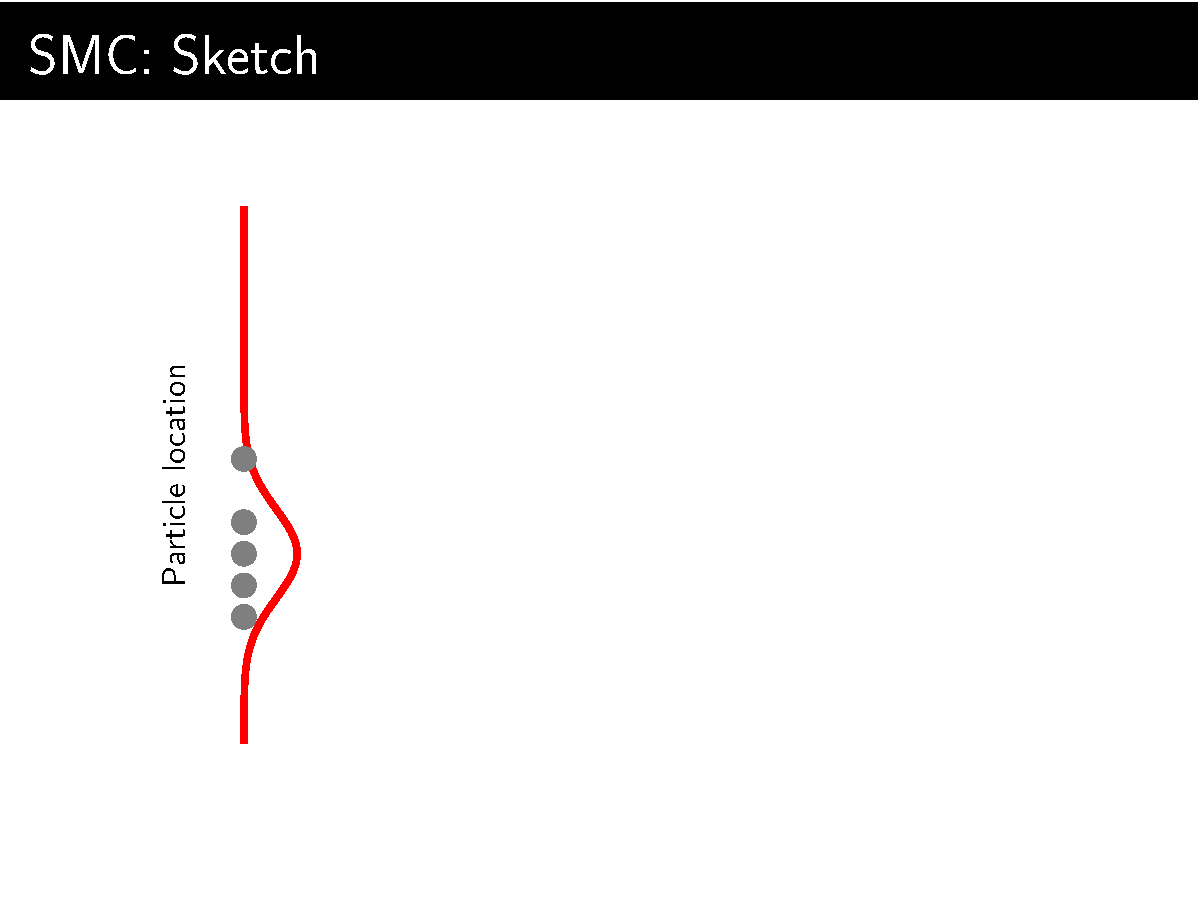
\includepdf[pages=-]{wonderful_smc_graphic_export}
%
%%%%%%%%%%%%%%%%%%%%%%%%%%%%%%%%%%%%%%%%%%
%\begin{frame}{Sequential Monte Carlo}
%Given distributions $P_0, ... P_N$ such that $\frac{P_i(x, \theta)}{P_{i+1}(x, \theta)}$ is computable
%\begin{itemize}
%\item Sample from a tractable proposal. 
%\end{itemize}
%
%\end{frame}
%
%
%%%%%%%%%%%%%%%%%%%%%%%%%%%%%%%%%%%%%%%%%%
%\begin{frame}{Likelihood-free Sequential Importance Sampling}
%
%From an earlier slide: "You need the ratios $\frac{P(x^{(i)}, \theta^{(i)})}{P(x^{(j)}, \theta^{(j)})} $ and
%$ \frac{Q(x^{(j)}, \theta^{(j)})}{Q(x^{(i)}, \theta^{(i)})}$." Not (quite) true.\\
%
%From the intro: "If you can't compute $\frac{P(x^{(i)}, \theta^{(i)})}{P(x^{(j)}, \theta^{(j)})} $, try to get the nasty part to appear in the proposal ratio."
%
%\end{frame}

%%%%%%%%%%%%%%%%%%%%%%%%%%%%%%%%%%%%%%%%%%
%\begin{frame}{}
%
%\centering 
%	%\only<1>{\vspace*{0cm}\hspace*{0cm}\includegraphics[scale=.2]{blah.eps}}\\
%%\footnote{Graphic: blah.com}
%
%\end{frame}

%%%%%%%%%%%%%%%%%%%%%%%%%%%%%%%%%%%%%%%%%

\begin{frame}[allowframebreaks]{Questions?}
\bibliography{prelim_biblio}
\begin{center}

 %\includegraphics[ trim={0cm 0cm 0 0},clip, width = .75\textwidth]{nice_things.jpeg}
\end{center}
\end{frame}
%%%%%%%%%%%%%%%%%%%%%%%%%%%%%%%%%%%

\end{document}